\begin{pastexam}[label={px:df3-098-ds-01}]{地方三等資訊處理 98 年 第一題}
（申論；18 分）

左下圖為一 6 × 6 迷宮，其中灰色區域表示不可通行，其餘可通行區域則有編號，入口與出口分別位於左上角
（編號 0）與右下角（編號 35）。假定每個區域有八個可能的行動方向，找尋出口路徑時，會依序嘗試此八個
方向（次序請參考右下圖之箭頭編號）。利用深度優先搜尋（depth-first search），在迷宮中探索所有可行
路徑（路徑中不可包含重複的區域）。
\begin{center}
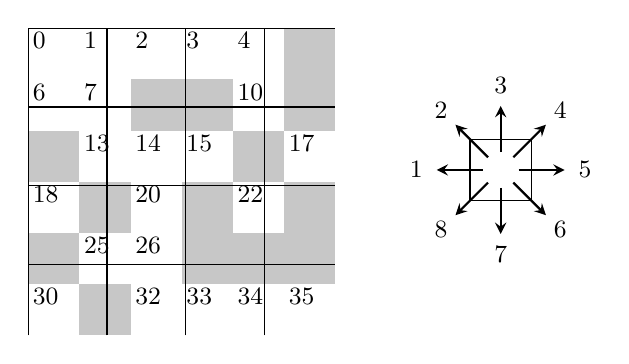
\begin{tikzpicture}[x=6.5mm, y=6.5mm]
\foreach \c in {5,8,9,11,12,16,19,21,23,24,27,28,29,31}{
  \pgfmathtruncatemacro{\r}{\c/6}
  \pgfmathtruncatemacro{\q}{\c-6*\r}
  \fill[black!22] (\q,-\r) rectangle (\q+1,-\r-1);
}
\foreach \c in {0,1,2,3,4,6,7,10,13,14,15,17,18,20,22,25,26,30,32,33,34,35}{
  \pgfmathtruncatemacro{\r}{\c/6}
  \pgfmathtruncatemacro{\q}{\c-6*\r}
  \node[anchor=north west, inner sep=1.5pt, font=\small] at (\q,-\r) {\c};
}
\draw (0,0) grid (6,-6);
\begin{scope}[xshift=60mm, yshift=-18mm, >=stealth, font=\small]
\draw (-0.6,-0.6) rectangle (0.6,0.6);
\foreach \a/\k in {180/1, 135/2, 90/3, 45/4, 0/5, -45/6, -90/7, -135/8}{
  \draw[->, thick] (\a:0.35) -- (\a:1.25);
  \node at (\a:1.65) {\k};
}
\end{scope}
\end{tikzpicture}
\end{center}
\begin{enumerate}[leftmargin=2.2em]
\item[㈠] 利用區域編號，寫出找到的第一條路徑（編號間用逗號隔開）。（4 分）
\item[㈡] 利用區域編號，寫出找到的倒數第二條路徑（編號間用逗號隔開）。（4 分）
\item[㈢] 找到第一條路徑前，曾經拜訪過但最後未出現在該路徑上之區域有那些？（利用區域編號作答）（5 分）
\item[㈣] 若迷宮大小改為 2 × 2，且所有區域均可通行，仍以左上角與右下角區域做為入口與出口，則共存在
多少種不同路徑？（5 分）
\end{enumerate}
\end{pastexam}

\begin{pastsoln}
\textbf{方向與搜尋方式。} 方向 1 到 8 依序是：西、西北、北、東北、東、東南、南、西南（從左邊
逆時針轉一圈）。 區域 $c$ 在第 $\lfloor c/6 \rfloor$ 列、第 $c \bmod 6$ 行，八個方向的鄰居編號
是 $c-1$、$c-7$、$c-6$、$c-5$、$c+1$、$c+7$、$c+6$、$c+5$（超出邊界的不算）。 這是回溯法
（資結書第~20.1~節）：從 0 開始，每到一個區域就照 1 到 8 的順序試每個方向，鄰居可以通行而且不在
目前的路徑上就走過去；走到 35 記下一條路徑，然後退回上一格試下一個方向；八個方向都試完就退回。

\textbf{㈠ 第一條路徑。} 從 0 出發，方向 1--4 都在邊界外，方向 5（東）是 1，一路往東：
\begin{itemize}
\item 0 → 1 → 2 → 3 → 4：每一格的方向 1--4 不是出界、就是已在路徑上，方向 5 往東可走。
\item 4：東邊 5 是灰色，東南 11 灰色，方向 7（南）是 10。
\item 10：方向 1 的 9 灰色，2、3 的 3、4 在路徑上，4、5 的 5、11 灰色，方向 6（東南）是 17。
\item 17：西 16、北 11 灰色，東邊出界，南 23 灰色，方向 8（西南）是 22。
\item 22：西 21 灰色，方向 2（西北）是 15；15 往西是 14，14 往西是 13。
\item 13：西 12 灰色，方向 2（西北）是 6，走進去：6 往東 7；7 的八個鄰居 6、0、1、2、14、13 在路徑上，
8、12 灰色，死路，退回 6；6 也沒有別的方向，退回 13。 方向 3（北）是 7，走進去：7 往西 6，
6 是死路，退回；7 也沒有別的路，退回 13。 方向 4 的 8 灰色，方向 5 的 14 在路徑上，方向 6
（東南）是 20。
\item 20：方向 1、5 灰色，2、3、4 的 13、14、15 在路徑上，方向 6 的 27 灰色，方向 7（南）是 26。
\item 26：西邊是 25。 25：西 24 灰色，方向 2（西北）是 18，18 的鄰居 13、25 在路徑上，其餘灰色或
出界，死路，退回 25；方向 3 的 19 灰色，4、5 的 20、26 在路徑上，方向 6（東南）是 32。
\item 32：西 31 灰色，西北 25、北 26 在路徑上，東北 27 灰色，方向 5（東）是 33，再往東 34、35。
\end{itemize}
第一條路徑：\textbf{0, 1, 2, 3, 4, 10, 17, 22, 15, 14, 13, 20, 26, 25, 32, 33, 34, 35}。

\textbf{㈡ 倒數第二條路徑。} 0 的鄰居依方向順序是 1（方向 5）、7（方向 6）、6（方向 7），所以
最後找到的那些路徑都從 0, 6 開始。 從 6 出發，同樣照方向順序，最後試的是 6 → 13（方向 6，東南；
方向 7 的 12 是灰色）。 13 的方向順序是 7（方向 3）、14（方向 5）、20（方向 6）、19 灰色（方向 7）、
18（方向 8），所以最後一批從 0, 6, 13, 18 開始。 18 只能往東南到 25；25 的方向順序是 20（方向 4）、
26（方向 5）、32（方向 6）、30（方向 8），30 是死路（鄰居 24、31 灰色，25 在路徑上），所以
最後找到的路徑經過 32。 32 的鄰居依序是 26（方向 3）、33（方向 5）：
\begin{itemize}
\item 先試 26：0, 6, 13, 18, 25, 32, 26, \dots。 26 的鄰居 20（方向 3）可以繞回上面，那些路徑先找到；
26 最後試方向 6 的 33，得到 0, 6, 13, 18, 25, 32, 26, 33, 34, 35。
\item 再試 33：0, 6, 13, 18, 25, 32, 33, 34, 35，這是最後一條。
\end{itemize}
所以倒數第二條路徑是 \textbf{0, 6, 13, 18, 25, 32, 26, 33, 34, 35}（最後一條是
0, 6, 13, 18, 25, 32, 33, 34, 35）。 這張迷宮一共有 2819 條不重複區域的路徑，都由 DFS 依序列舉。

\textbf{㈢ 找到第一條路徑前拜訪過、但不在第一條路徑上的區域：6, 7, 18。} ㈠ 的過程裡，從 13
往西北進入 6、再到 7（死路），又從 13 往北進入 7、再到 6（死路）；從 25 往西北進入 18（死路）。
其他拜訪過的區域都在第一條路徑上。

\textbf{㈣ 2 × 2 迷宮：5 條。} 四格編號 0、1（上排）、2、3（下排），八個方向下任兩格都相鄰。
從 0 到 3、不重複經過區域的路徑，看中間經過哪些格：
\begin{itemize}
\item 不經過中間格：0, 3（1 條）；
\item 經過一格：0, 1, 3 與 0, 2, 3（2 條）；
\item 經過兩格：0, 1, 2, 3 與 0, 2, 1, 3（2 條）。
\end{itemize}
共 $1 + 2 + 2 = 5$ 條。 照 DFS 的方向順序找到的順序是 0,1,3；0,1,2,3；0,3；0,2,1,3；0,2,3。
\end{pastsoln}
